\documentclass[border=10pt]{standalone}

\usepackage{tikz}
\usepackage{tikzsymbols}
\usetikzlibrary{calc,patterns,shapes.geometric}

\def\centerarc[#1](#2)(#3:#4:#5){\draw[#1] ($(#2)+({#5*cos(#3)},{#5*sin(#3)})$) arc (#3:#4:#5);}

\begin{document}
	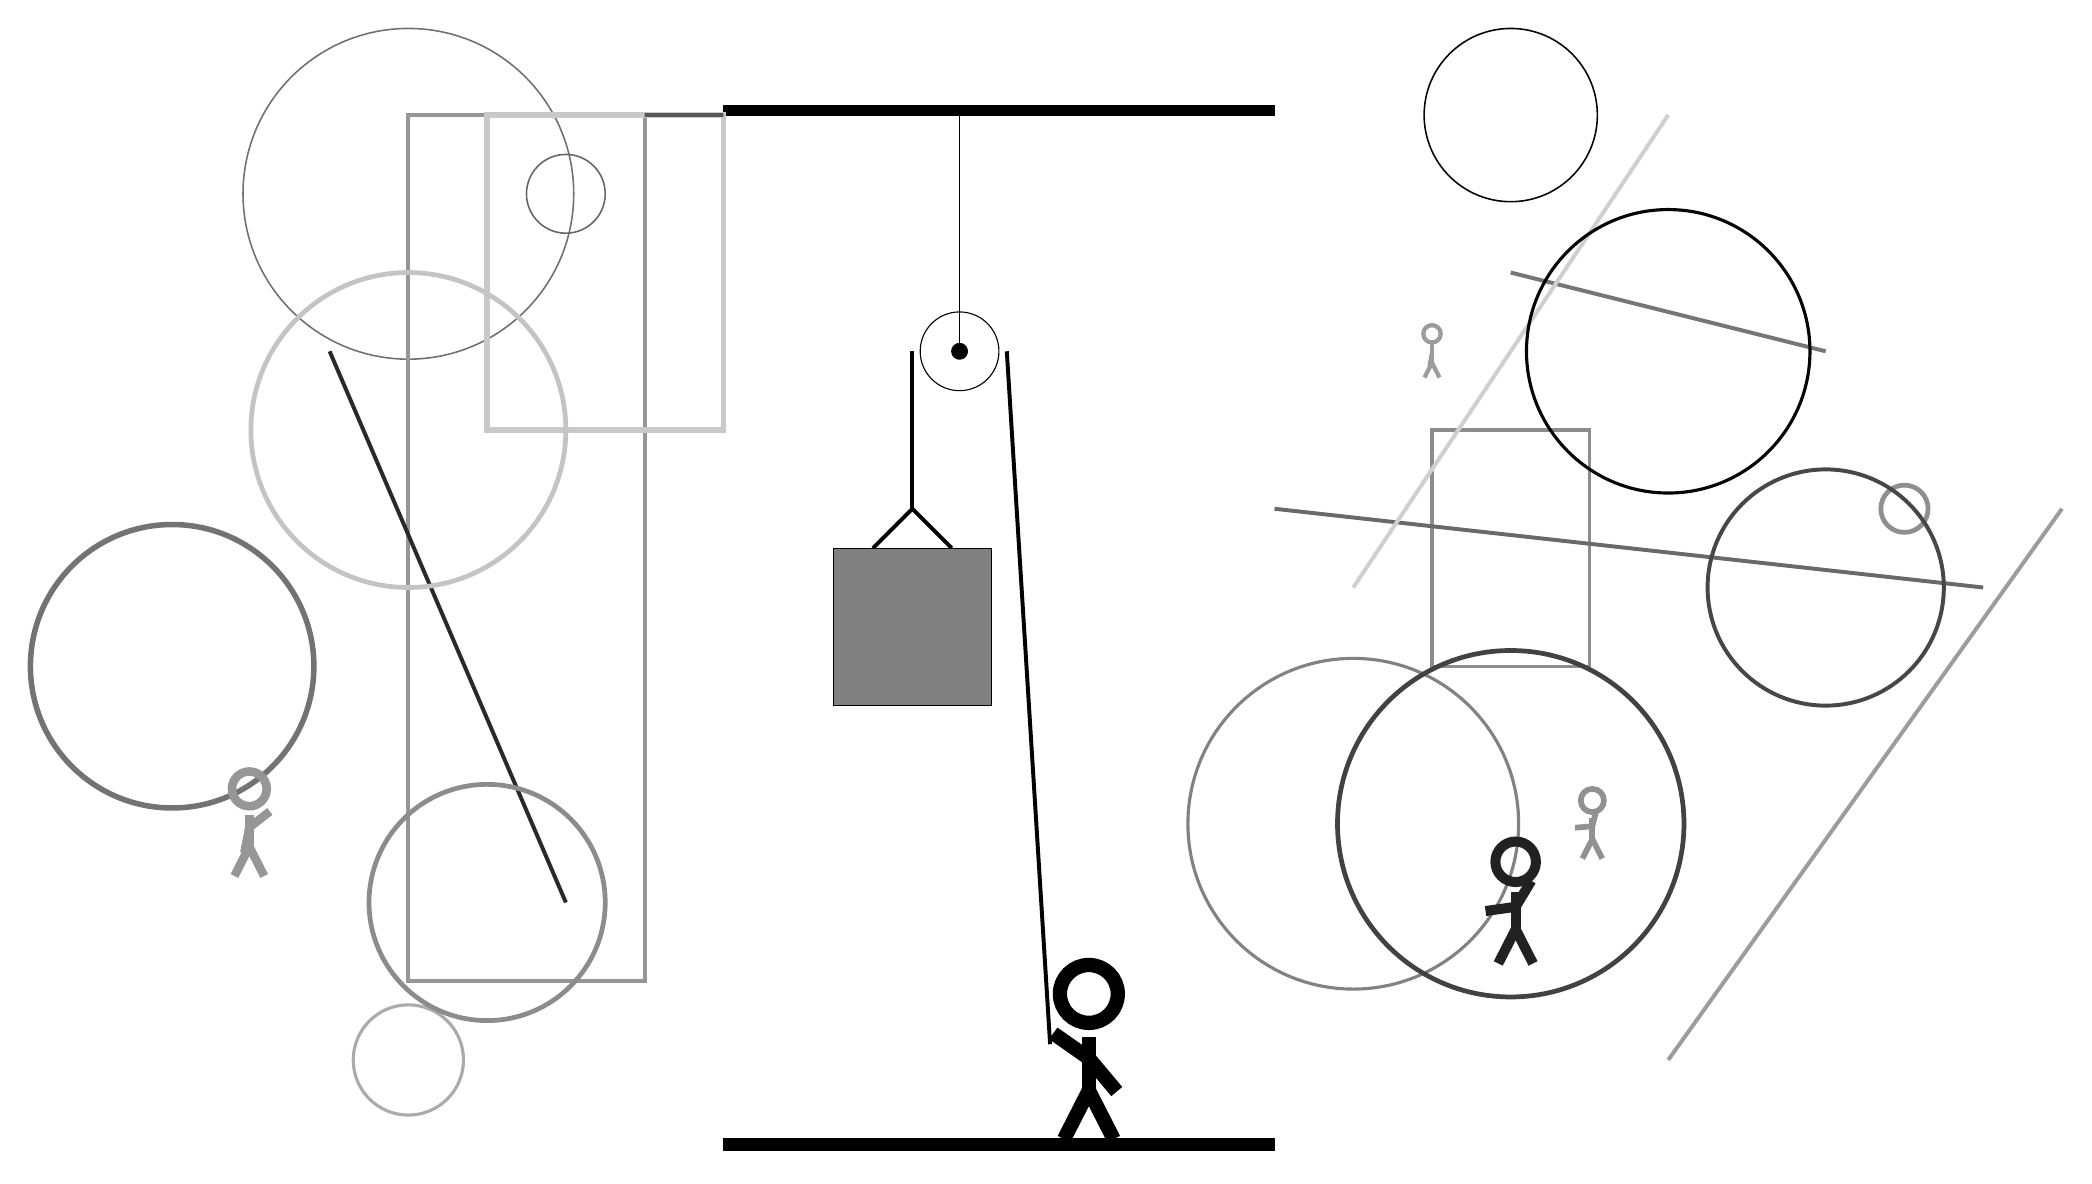
\begin{tikzpicture}
		%%%%% START %%%%%
		
		\draw[fill=black] (-2, 10) rectangle (5, 10.125);
		
		\draw (1, 7) circle (0.5);
		\draw[fill=black] (1, 7) circle (0.1);
		\draw (1, 10) -- (1, 7);
		
		\draw[line width=0.5mm] (-0.1, 4.5) -- (0.4, 5.0) -- (0.9, 4.5);
		\draw[fill=black!50] (-0.6, 4.5) rectangle (1.4, 2.5);
		
		\draw[line width=0.5mm] (0.4, 7) -- (0.4, 5.0);
		\centerarc[line width=0.5mm](1, 7)(0:180:0.6);
		\draw[line width=0.5mm](1.6, 7) -- (2.15, -1.8);
		
		\draw [line width=0.2mm, color=black!56](-6, 9) circle (2.1);
		
		\draw [line width=0.2mm, color=black!98](8, 10) circle (1.1);
		\draw[line width=0.5mm, color=black!41] (-3, -1) rectangle (-6, 10);
		\draw[line width=0.5mm, color=black!39](10, -2) -- (15, 5);
		
		\draw [line width=0.4mm, color=black!33](-6, -2) circle (0.7);
		\node[line width=0.5mm, color=black!43] at (9, 1) {\Strichmaxerl[4][5][76]};
		\draw [line width=0.6mm, color=black!44](13, 5) circle (0.3);
		
		\draw[line width=0.5mm, color=black!54](8, 8) -- (12, 7);
		\draw[line width=0.5mm, color=black!84](-7, 7) -- (-4, 0);
		
		\draw[line width=0.4mm, color=black!45] (7, 3) rectangle (9, 6);
		\draw[line width=0.5mm, color=black!59](5, 5) -- (14, 4);
		\draw [line width=0.4mm, color=black!49](6, 1) circle (2.1);
		\draw [line width=0.7mm, color=black!55](-9, 3) circle (1.8);
		
		\draw [line width=0.6mm, color=black!74](8, 1) circle (2.2);
		\draw[line width=0.7mm, color=black!21] (-2, 6) rectangle (-5, 10);
		\draw [line width=0.6mm, color=black!45](-5, 0) circle (1.5);
		
		\draw[line width=0.5mm, color=black!66] (-3, 10) rectangle (-2, 10);
		\draw [line width=0.2mm, color=black!60](-4, 9) circle (0.5);
		\draw [line width=0.6mm, color=black!23](-6, 6) circle (2.0);
		
		\draw[line width=0.5mm, color=black!19](10, 10) -- (6, 4);
		\node[line width=0.3mm, color=black!41] at (-8, 1) {\Strichmaxerl[6][79][38]};
		
		\node[line width=0.6mm, color=black!39] at (7, 7) {\Strichmaxerl[3][79][90]};
		\draw [line width=0.4mm, color=black!98](10, 7) circle (1.8);
		\draw [line width=0.5mm, color=black!72](12, 4) circle (1.5);
		\node[line width=0.6mm, color=black!87] at (8, 0) {\Strichmaxerl[7][8][59]};
		
		
		\node at (2.6, -1.9) {\Strichmaxerl[10][-35][-50]};
		
		\draw[fill=black] (-2, -3) rectangle (5, -3.15);
		
		%%%%% END %%%%%
	\end{tikzpicture}
\end{document}